\documentclass[
  a4paper,            % DIN A4
  DIV=10,             % Schriftgröße und Satzspiegel
  oneside,            % einseitiger Druck
  BCOR=5mm,           % Bindungskorrektur
  parskip=half,       % Halber Abstand zwischen Absätzen
  numbers=noenddot,   % Kein Punkt hinter Kapitelnummern
  bibtotoc,           % Literaturverzeichnis im Inhaltsverzeichnis
  listof=totoc        % Abbildungs- und Tabellenverzeichnis im Inhaltsverzeichnis
]{scrartcl}
\usepackage{../style/termpaperstyle}

%\usepackage{layout}       % Layout Debugging
%\usepackage{showframe}    % Layout Debugging
\usepackage{lipsum}       % for example only
\usepackage{blindtext}    % for example only


\begin{document}
% !TEX root = ../termpaper.tex
%
% configurations
%

% text field
%-> replace supervisor names with correct ones
\firstSupervisor{Prof. Dr. Franz Schubert}
\secondSupervisor{}    % only if needed, otherwise left blank

% text field
%-> replace title with your title of the seminar work
\termPaperTitle{Solarbetriebene, mobile Wetterstation}
\termPaperTitleEN{}

% text field
%-> replace the key words with your own key words or remove the words
\keywordsDE{Leben, Universum, Alles}
\keywordsEN{Life, Universe, Everything}

% text field
%-> replace jon with your name
\termPaperAuthor{Isabell Albrecht, Erik Engelhardt, Oliver Kochan, Florian Steffens}

% text field
%-> enter the submission date
\submissionDate{13. Januar 2019}

% switch - uncomment only one
%-> uncomment NDA or public
%\NDA{yes}
\NDA{no}

%-> uncomment cover or cover Corporate Design 2017
%\Cover{CD2017}
%\Cover{CD2017NoLogo}
\Cover{Std2018}

% switch - uncomment only one
%-> uncomment the kind of seminar you are in
\seminarKind{S}     % seminar in bachelor course
%\seminarKind{Pro}   % pro-seminar in bachelor course
%\seminarKind{GSem}  % foundation seminar in master computer science
%\seminarKind{HSem}  % main seminar in master computer science


% switch - uncomment only one
%-> uncomment the study course you are in
%\studycourse{TI}
%\studycourse{AI}
%\studycourse{WI}
%\studycourse{EI}
%\studycourse{BMT}
%\studycourse{MAI}  % master in computer science
%\studycourse{MIK}
%\studycourse{MA}
\studycourse{MES}  

    % load all settings

%\layout{}                 % Layout Debugging

\hyphenation{Ba-che-lor-the-sis Mas-ter-the-sis}

% Cover page here, no page number
\ICoverPage

% Titlepage is page one even if the number is not shown.
\pagenumbering{roman}

% Table of contents here
\newpage
\tableofcontents

% Uncomment if list of source code is needed (rarely).
%\lstlistoflistings  % requires package listings, needs to uncommenting of usepackage

% path to the chapters folder is set to find the images used there
\graphicspath{ {./img/} }

% Chapters
\clearpage
\pagenumbering{arabic}

\begin{abstract}
% !TEX root = ../termpaper.tex
% first example for the abstact
% @author Thomas Lehmann
%
\vspace*{0.4cm}

\noindent Der vorliegende Text ist ein Beispiel für eine Seminararbeit und soll nur die Verwendung des Templates aufzeigen.

\end{abstract}

\ITextBlockKeywords

% !TEX root = ../termpaper.tex
% first example section
% @author Thomas Lehmann
%

\section{Einleitung}

% Add additional chapters here
\section{Spannungsversorgung}\label{sec.spannungsversorgung}
In diesem Abschnitt soll auf die hardwareseitige Umsetzung der Spannungsversorgung für die Wetterstation eingegangen werden. Ziel ist der Entwurf einer Platine, auf der sämtliche Anforderungen umgesetzt werden.

\subsection{Anforderungen}\label{subsec.anforderungen}
Zunächst sollen in diesem Abschnitt die Anforderungen, die sich aus der Aufgabenstellung ableiten lassen, sowie solche, die sich aus den weiteren Überlegungen zur Umsetzung der Wetterstation ergeben.

\begin{itemize}

	\item Messung des Ladestroms
	\item Messung der Batteriespannung (Ladezustand)
	\item Messung des Stromverbrauchs der Wetterstation

\end{itemize}

Des Weiteren soll der Stromverbrauch der Wetterstation so niedrig wie möglich sein, um die Puffer-Batterie zu schonen und sonnenarme Phasen bzw. die Nacht ohne Stromausfall überbrücken zu können. Die verwendete Batterie hat eine Ladeschlussspannung von 12\,V. Da für den Mikrocontroller und die Sensoren allerdings Spannungspegel von 3,3\,V und 5\,V benötigt werden, müssen diese auf der Platine erzeugt werden.

Aus den mechanischen Anforderungen, dass Mikrocontroller, Platine und Sensoren möglichst in einem Gehäuse untergebracht werden sollen, ergibt sich, dass die entworfene Platine auf die Pinheader des Mikrocontrollers gesteckt werden soll.

\subsection{Erzeugung benötigter Spannungen}\label{subsec.Spannungserzeugung}
Wie in \ref{subsec.anforderungen} beschrieben, werden sowohl 3,3V als auch 5V-Pegel für die Wetterstation benötigt. Angestrebt ist, dass die verwendeten Buck-Spannungsregler eine möglichst geringe Ruhestromaufnahme und einen guten Wirkungsgrad haben. Die Wahl fiel hierbei auf den \textit{LTC3621}. Dieser hat einen Eingangsspannungsbereich von 2,7\,V bis 17\,V und eine Ausgangsspannung, die sich über einen Spannungsteiler am Feedback-Pin zwischen 0,6\,V und der Eingangsspannung einstellen lässt. Der Ruhestrom beträgt laut Datenblatt 3,5\,$\mu$A ~\cite{ltc3621}. Der Regler kann einen maximalen Ausgangsstrom von 1\,A liefern. Da bei der Wahl des Spannungsreglers noch keine Werte über die von der Peripherie benötigte Leistung vorlag, ist dieser Wert eventuell etwas überdimensioniert.

Die Beschaltung des Reglers entspricht den Empfehlungen des Datenblatts, wie sie in Abbildung \ref{fig.ltc3621} dargestellt ist:

\begin{figure}[H]
  \centering
  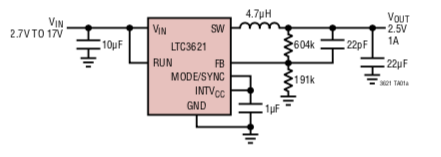
\includegraphics[width=0.6\textwidth]{./img/ltc3621.png}
  \caption{Darstellung des LTC3621 mit beispielhafter Beschaltung gemäß Datenblatt~\cite{ltc3621}}\label{fig.ltc3621}
\end{figure}

Zusätzlich verfügt dieser Regler über die Option, über einen Befehl des Mikrocontrollers manuell ein- bzw. ausgeschaltet zu werden, was weiterhin günstig für den Gesamtstromverbrauch ist.

\subsubsection{3V3}\label{subsubsec.3v3}
Im folgenden soll hauptsächlich auf die Dimensionierung des Spannungsteilers zur Erzeugung von 3,3\,V eingegangen werden. Der Regler hat dabei eine interne Referenzspannung am FB-Pin, die 0,6\,V beträgt, über die die Ausgangsspannung geregelt wird. 

\begin{figure}[H]
  \centering
  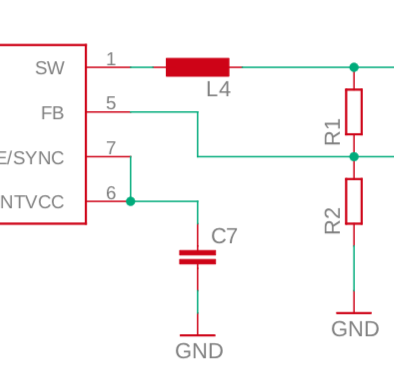
\includegraphics[width=0.4\textwidth]{./img/spannungsteiler_3v3.png}
  \caption{Spannungsteiler am FB-Pins des 3V3 Reglers}\label{fig.spgsteiler3v3}
\end{figure}

Es kann somit der folgende Spannungsteiler aufgestellt werden:

\begin{minipage}{\textwidth}
\begin{equation}\label{eq:Spannungsteiler3v3}
\frac {U_{FB}}{U_a}{=}  \frac{R_{101}}{R_{101}+R_{100}}
\end{equation}
\end{minipage}

Mit $U_{FB}=0,6\,\si{\volt}$, $U_a=3,3\,\si{\volt}$ und $R_{101}=150\,\si{\kilo\ohm}$ ergibt sich:

\begin{minipage}{\textwidth}
\begin{equation}\label{eq:Spannungsteiler3v3b}
\frac {0,6\,\si{\volt}}{3,3\,\si{\volt}}{=}  \frac{150\,\si{\kilo\ohm}}{150\,\si{\kilo\ohm}+R_{100}} \Rightarrow R_{100}=680\,\si{\kilo\ohm}
\end{equation}
\end{minipage}

Der Spannungsteiler wurde hochohmig dimensioniert, um den Stromfluss möglichst klein zu halten.


%Spannungsteiler Formel, was wird alles von 3V3 versorgt 
\subsubsection{5V}\label{subsubsec.5v}
Die Bestimmung des Spannungsteilers für die Erzeugung von 5V erfolgt analog zu Abschnitt \ref{subsubsec.3v3}. Es lässt sich folgender Spannungsteiler aufstellen:

\begin{figure}[H]
  \centering
  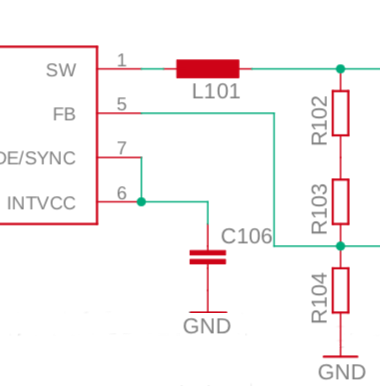
\includegraphics[width=0.4\textwidth]{./img/spannungsteiler_5v.png}
  \caption{Spannungsteiler am FB-Pins des 5V Reglers}\label{fig.spgsteiler5v}
\end{figure}

Dieser wird beschrieben durch:

\begin{minipage}{\textwidth}
\begin{equation}\label{eq:Spannungsteiler5v}
\frac {U_{FB}}{U_a}{=}  \frac{R_{104}}{R_{104}+R_{103}+R_{102}}
\end{equation}
\end{minipage}

Mit $U_{FB}=0,6\,\si{\volt}$, $U_a=3,3\,\si{\volt}$ und $R_{104}=100\,\si{\kilo\ohm}$ ergibt sich:

\begin{minipage}{\textwidth}
\begin{equation}\label{eq:Spannungsteiler5vb}
\frac {0,6\,\si{\volt}}{3,3\,\si{\volt}}{=}  \frac{100\,\si{\kilo\ohm}}{10\,\si{\kilo\ohm}+R_{103}+R_{102}} \Rightarrow R_{103}=680\,\si{\kilo\ohm}; R_{102}=47\,\si{\kilo\ohm}
\end{equation}
\end{minipage}



\subsection{Spannungsabschaltung}\label{subsec.Spannungsabschaltung}
Im Zuge der Überlegungen bezüglich möglicher Energiesparmaßnahmen wurden sowohl das Bluetooth- als auch das GPS-Modul als große Verbraucher ermittelt. Da beide Module auch nicht dauerhaft benötigt werden -- das GPS-Modul nur alle 15 Minuten zur Neuausrichtung des Panels und das Bluetooth-Modul nur nach Bedarf -- ist es sinnvoll, die Betriebsspannungen beider Module schaltbar zu machen. Eine Möglichkeit dafür ist die Verwendung eines p-Kanal-Mosfets, der von einem n-Kanal-Mosfet getrieben wird. Diese Schaltung wird in Abbildung \ref{fig.spgsabschaltung} dargestellt.

\begin{figure}[H]
  \centering
  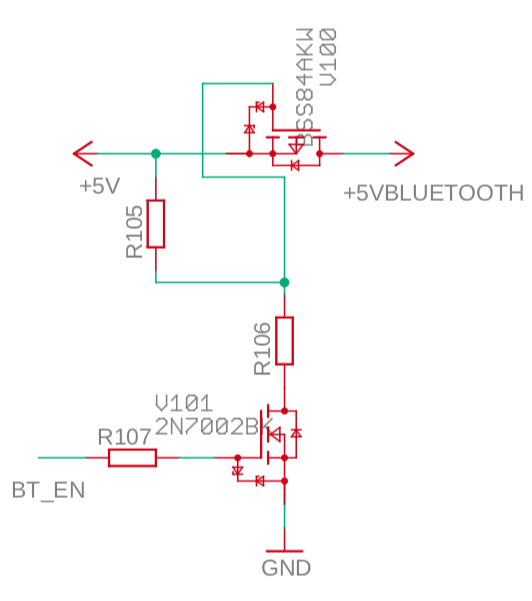
\includegraphics[width=0.4\textwidth]{./img/spannungsabschaltung.png}
  \caption{Spannngsabschaltung Bluetooth-Modul}\label{fig.spgsabschaltung}
\end{figure}

Bei einem Einschaltsignal über BT\_EN vom Mikrocontroller schaltet der n-Kanal-Mosfet V101 durch; der Spannungsteiler aus $R_{105}$ und $R_{106}$ ist aktiv. Es sei $R_{105}=100\,\si{\kilo\ohm}$ und $R_{106}=1\,\si{\kilo\ohm}$. Daraus ergibt sich für die Gate-Source-Spannung des p-Kanal-Transistors $U_{GS}$:

\begin{minipage}{\textwidth}
\begin{equation}\label{eq:UGS}
{U_{GS}}{=} 5\,\si{\volt}-5\,\si{\volt}\cdot \frac{1\,\si{\kilo\ohm}}{101\,\si{\kilo\ohm}}{=}4,95\,V
\end{equation}
\end{minipage}

Damit schaltet der p-Kanal-Transistor mit $U_{GS,th}=1,6\,V$ sicher durch.
Die Schaltung für das GPS-Modul wird analog dazu entworfen.


\subsection{Messung Strom/Spannung}\label{subsec.MessungStromSpannung}
Aus den Anforderungen abgeleitet wird auf der Platine die Messung von Strom und Spannung implementiert. Für die Messung der Stromaufnahme werden zwei Stromsensoren vom Typ ACS172 verwendet. Diese messen den Ladestrom der Batterie und die Stromaufnahme des Boards und geben diese Werte an den Mikrocontroller.
Die Spannungsmessung wird mit einem einfachen Spannungsteiler umgesetzt, sodass bei $U_{Bat}=12\,\si{\volt}$ 3,3\,V nicht überschritten werden. Mit $R_{109}=270\,\si{\kilo\ohm}$ und $R_{110}=100\,\si{\kilo\ohm}$ ergibt sich eine maximale Spannung von 3,24\,V.







\section{Ausrichtung des Solarpanels}\label{sec:ausrichtung des Solarpanels}
Um die Leistungsaufnahme des Solarpanels zu optimieren ist es notwendig dieses direkt auf die Sonne auszurichten und diese Ausrichtung auch in geeigneten Zeitabständen zu korrigieren. Im Vergleich mit einem fest ausgerichteten Solarpanel konnten J. Rizek \emph{et al.} mit einem nachgeführten Solarpanel beispielsweise die Leistungsaufnahme um durchschnittlich 30\% erhöhen~\cite{Rizek2008}.

Hierfür kommen grundsätzlich verschiedene Methoden in Frage. In diesen Fall soll die Position der Sonne relativ zur Wetterstation auf Grundlage des Längen- und Breitengrades, der Uhrzeit und des Kalendertages berechnet werden. Diese Information werden über das GPS-Modul bereitgestellt. Anschließend wird das Solarpanel mit Hilfe der Motoren, des Kompass-Moduls und des, am Panel befestigten Neigungssensors, auf die Sonne ausgerichtet.

\subsection{Berechnung der Sonnenposition}\label{sec:berechnung_der_sonnenposition}
Da die Formeln zur Berechnung der Sonnenposition in diesem Projekt lediglich benutzt werden wird an dieser Stelle auf eine Herleitung verzichtet. Die verwendeten Formeln können beispielsweise im \emph{Astronomical Almanac}~\cite{Anon1984} gefunden werden. \emph{M. L. Roderick} beschreibt die nötigen Berechnungen in seinem Report~\cite{Roderick1992} und liefert zudem compilierbaren C-Code. Dieser wird im folgenden zur Berechnung der Sonnenposition verwendet.

Die Position der Sonne im Bezug auf einen Beobachter auf der Erde lässt sich durch die Werte \emph{Zenith} und \emph{Azimut} eindeutig beschreiben. Der Zenith beschreibt den Winkel zwischen einer Linie vom Beobachter zur Sonne und der Vertikalen. Der Azimut den Winkel zwischen der Horizontalen und Norden. Dabei stehen beispielsweise ein Azimut von \SI{90}{\degree} für Osten, \SI{180}{\degree} für Süden und \SI{270}{\degree} für Westen. Eine Veranschaulichung kann in Abbildung~\ref{fig:zen_azi} gefunden werden.

\begin{figure}[H]
  \centering
  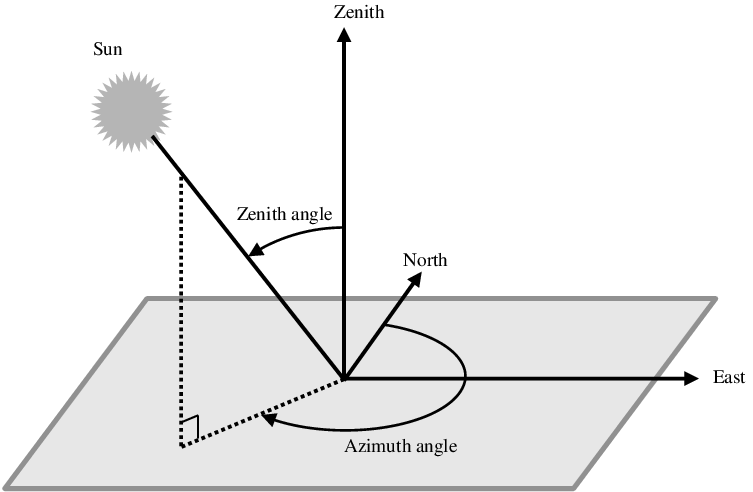
\includegraphics[width=\textwidth]{./img/Representation-of-azimuth-and-zenith-angles.png}
  \caption{Beschreibung der Sonnenposition durch Zenith und Azimut~\cite{Nou2016}}\label{fig:zen_azi}
\end{figure}

Die Genauigkeit der verwendeten Formeln beträgt laut dem \emph{Astronomical Almanac} 


%%% Local Variables:
%%% mode: latex
%%% TeX-master: "../termpaper"
%%% End:


%\bibliographystyle{plain}
\bibliographystyle{dinat}
\bibliography{literature}

%\Istatement

\end{document}

%%% Local Variables:
%%% mode: latex
%%% TeX-master: t
%%% End:
